\chapter{Algorithm}
	Starting out, I did some research into horizontal and vertical edge detection by going back and looking through the old slides on the subject, reading in the book, reading the opencv documentation, to understand how their version works, and doing general knowledge search on the Internet.\\
	\\
	An edge is defined as a sudden jump in intensity in an image. Imagine the simple graph in \autoref{fig:sobelGraph}, it illustrates the hypothetical image with an intensity jump, in the algorithm this should be seen as an edge.
	
	\begin{figure}[H]
		\centering
		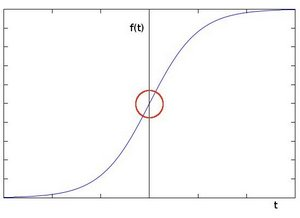
\includegraphics[width=0.4\linewidth]{figure/sobelGraph}
		\caption{Simple representation of a hypothetical intensity jump in an image. Taken from opencv documentation for the sobel function.}
		\label{fig:sobelGraph}
	\end{figure} 
	
	Doing simple edge detection involves making two 3x3 kernels; one for horizontal and one for the vertical axis. As the assignment called for a gray scale image, the image will have to be converted to gray scale, or a gray image have to be used. The kernels that worked the best for me, looked like this:
	
	\[
	xKernel = 
	\begin{bmatrix}
		1 & 0 & -1\\
		2 & 0 & -2\\
		1 & 0 & -1
	\end{bmatrix},\hspace{0.7cm}
	yKernel = 
	\begin{bmatrix}
	1 & 2 & 1\\
	0 & 0 & 0\\
	-1 & -2 & -1
	\end{bmatrix}
	\]
	In theory a larger kernel could be used, as long as it is an odd size. If a larger kernel is used though, the resulting edges will be thicker.
	These two kernels are then individually convolved with image, this calculates the approximate derivative. The resulting two images, will be called xGradient and yGradient. These images are now already showing respectively horizontal and vertical edges.\newpage
	At each point of the image, we have to calculate the approximate of the gradient at that point. This is done by essentially combining the results of the two earlier convolutions. This is done by taking the following formula:
	\[
	finalGradient = \sqrt{xGradient^2+yGradient^2}
	\]
	This will be the resulting final gradient, which in turn also will show both the horizontal and vertical edges in the original image.\\
	\\
	So the resulting algorithm in steps will be:
	\begin{enumerate}
		\item Load image
		\item Make kernels
		\item Convolve image with x kernel
		\item Convolve image with y kernel
		\item Take the resulting two gradients and take the approximate gradient of them combined into one final image
		\item (Optional) Have a Tuborg to celebrate
	\end{enumerate}